\documentclass[10pt,a4paper]{article}
\usepackage[top=1in, bottom=1in, left=1in, right=1in]{geometry}
\usepackage[utf8]{inputenc}
\usepackage{amsmath}
\usepackage{amsfonts}
\usepackage{amssymb}
\usepackage{amsthm}
\usepackage{microtype} 
\usepackage{graphicx}
\usepackage{capt-of}
\usepackage{abstract}
\usepackage{hyperref}
\usepackage{url}
\usepackage{placeins}
\usepackage{bm}
\usepackage{xcolor}
\usepackage{paralist}

\usepackage{array}
\newcolumntype{L}[1]{>{\raggedright\let\newline\\\arraybackslash\hspace{0pt}}m{#1}}
\newcolumntype{C}[1]{>{\centering\let\newline\\\arraybackslash\hspace{0pt}}m{#1}}
\newcolumntype{R}[1]{>{\raggedleft\let\newline\\\arraybackslash\hspace{0pt}}m{#1}}

\newcommand{\Mod}[1]{\ (\mathrm{mod}\ #1)}
\newcommand\maybegeq{\stackrel{?}{\geq}}

\usepackage[backend=biber]{biblatex}

\newtheorem{lemma}{Lemma}

\graphicspath{ {./images/} }

\pagenumbering{empty}

\title{Collatz tree decomposed}
\author{Markus Macher \\ email \href{mailto:markus.macher@gmail.com}{markus.macher@gmail.com}} 
\begin{document}
\renewcommand{\abstractname}{Abstract}
\begin{abstract}
By decomposing the Collatz tree into a two-dimensional odd-even relation we show that it is sufficient to consider odd numbers (or a subset of even numbers) only using graph theory. A simple set of equations is used to build a connection graph which shows that all odd numbers are connected. We show that any valid proof that shows that all odd numbers (or a subset of even numbers) are connected without knowing their exact relation automatically proves the Collatz conjecture. Reasonable solutions solving the graph using graph theory or linear algebra are suggested.
\end{abstract}
\noindent
\bigskip\bigskip\bigskip
\noindent
\pagenumbering{arabic}

%-----------------------------------------------------------------------------
\section{Introduction}
%-----------------------------------------------------------------------------
We start by describing that the even and odd numbers of the Collatz tree can be separated into a two-dimensional odd-even relation. The roles of odd numbers and subsets of even numbers are shown. Using that separation, we show that any possibly separated tree of odd numbers has to contain exactly one loop which implicates that, if all odd numbers are connected, the Collatz tree is built.
Finally, a simple set of equations is used to build a network diagram with endpoints. The diagram and the equation set suggest that a solution should be possible using graph theory, rotation-shift-operations in 2D or similar operations in 3D.
%-----------------------------------------------------------------------------
\section{The reverse path}
%-----------------------------------------------------------------------------
The reverse path is built by $2$ operations, implicated by the Collatz rules.

We define
\begin{equation}
M(x)=2\cdot x
\end{equation}
which must be applied on any new number because it leads to an even number.

We define
\begin{equation}
D(x)=\frac{(x-1)}{3}
\end{equation}
which must be applied on any new even number when the operation leads to an (odd) integer.

In the reverse path, every $D$ splits the way into 2 paths. $A_k$ shall be the indexed set of all integers on which $D$ can be applied.
The path starts at 1, which is multiplied by 2 infinitely often. On its way up, on every $A_k$ the way is split. While $A_k$ is further multiplied, the second way leads to an odd number. This odd number is, like the 1, multiplied by 2 infinitely often hitting other $A_k$ on its way.
%-----------------------------------------------------------------------------
\section{Properties of even numbers}
%-----------------------------------------------------------------------------
The set of even numbers can be split into 3 sets each indexed with $k=0,1,2,\ldots$:
\begin{equation}
 \begin{cases}
	 6k+4 & \text{set of even numbers } A_k \text{ that solve } D(A_k) \\
	 6k+2 & \text{intermediary numbers between two } A_k \\
	 6k+6 & \text{multiples of 3}
 \end{cases}
\label{eq:6kcases}
\end{equation}
%-----------------------------------------------------------------------------
\subsection{Properties of $A_k$}
%-----------------------------------------------------------------------------

We define the set of even integers (only even integers are allowed) on which $D$ can be applied as
\begin{equation}
A_k=6k+4
\label{eqAkdef}
\end{equation}
with $k\ge0$. So, they are 4,10,16,22,$\ldots$.

By applying $D$, we get the set of odd integers:
\begin{equation}
N_k=D(A_k)=2k+1
\label{eqNk}
\end{equation}

We can make the following statements:
\begin{lemma}
$D$ is a bijective function between $A_k$ and the set of all odd integers $N_k$.
\end{lemma}
\begin{lemma}
Each odd number $N_k$ reached by $D(A_k)$ builds a new independent branch by multiplying by 2 infinitely often.
\end{lemma}
\begin{table}[!htb]
\centering
\begin{tabular}{|r|r|}
\hline
	Decimal & Binary \\
\hline
	40 & 101000 \\
	20 & 10100 \\
	10 & 1010 \\
	5 & 101 \\
\hline
\end{tabular}
\caption{Binary decomposition}
\label{table:binary_decomp}
\end{table}
This follows from the fact that dividing back to the odd number is a unique path. In binary notation it can be seen that the odd number $N_k$ is always present and a right-shift has to stop at the rightmost $1$ (Table \ref{table:binary_decomp}).

\begin{lemma}
Together with the odd numbers, $\mathbb{N}_+$ is built by $M$-operations.
\label{lemma:nplus}
\end{lemma}
This follows from the fact that any even number can be divided by 2 to finally reach an odd number.

%-----------------------------------------------------------------------------
\subsection{Intermediary numbers}
%-----------------------------------------------------------------------------
Intermediary numbers are even numbers that are between the double multiplication of two $A_k$ (Lemma \ref{lemma:AkAl}). They can be expressed as
\begin{equation}
I_k=6k+2=2,8,14,\ldots
\end{equation}
and can never be an $A_k$ because
\begin{equation}
D(I_k)=\frac{6k}{3}+\frac{1}{3}=2k+\frac{1}{3}
\end{equation}
never is an integer.
%-----------------------------------------------------------------------------
\subsection{Multiples of 3}
%-----------------------------------------------------------------------------
Even numbers that are multiples of 3 are
\begin{equation}
J_k=6k+6=6,12,18,\ldots
\end{equation}

They can never be an $A_k$ because
\begin{equation}
D(J_k)=\frac{6k+6}{3}-\frac{1}{3}=2k+2-\frac{1}{3}
\end{equation}
never is an integer.

%-----------------------------------------------------------------------------
\section{Multiplication of $A_k$ by $2^n$}
%-----------------------------------------------------------------------------
Multiplying $A_k$ by $2^n$ can be viewed as
\begin{equation}
2^n\cdot A_k=2^n\cdot6k+2^n\cdot4-4+4=6\cdot(2^n k+\frac{2}{3}\cdot2^n-\frac{2}{3})+4
\end{equation}
The expression
\begin{equation}
\frac{2}{3}\cdot2^n-\frac{2}{3}=2\cdot\frac{2^n-1}{3}
\end{equation}
contains Mersenne numbers which can be divided by 3 when $n$ is an even number. So we can make the following statement:

\begin{lemma}
For any $k$, $2^n\cdot A_k$ with even number $n=2,4,6,\ldots$ leads to another $A_l$ with $l$ being an even number.
\label{lemma:AkAl}
\end{lemma}
\begin{equation}
A_{l}=6\cdot(2^nk+2\cdot\frac{2^n-1}{3})+4
\end{equation}
Between two $A_k$, there are intermediary even numbers $2^n\cdot A_k$ with $n=1,3,5,\ldots$.

Lemma \ref{lemma:AkAl} is a statement about the relation between $A_k$ and $A_l$ only and not about the position of the first appearing $A_k$ in the branch started from an odd number.

%-----------------------------------------------------------------------------
\section{Relation between even and odd numbers}
%-----------------------------------------------------------------------------
The general formula to reach an odd integer $N_k=2k+1$ from another odd integer $N_g=2g+1$ in the reverse path is
\begin{equation}
	N_k=\frac{N_g\cdot2^n - 1}{3}
\label{eq:geneq}
\end{equation}
or
\begin{equation}
	2k+1=\frac{(2g+1)\cdot2^n - 1}{3}
\label{eq:geneqkg}
\end{equation}
or
\begin{equation}
	6k+4=(2g+1)\cdot2^n
\label{eq:Ak_vs_all}
\end{equation}
with $n=1,2,3,\ldots$, because for $n=0$ we would apply the $D$-operation to the odd number $N_g$.

The left side of Eq. \ref{eq:Ak_vs_all} is the set of $A_k$.
The right side is $\mathbb{N}_+$ (Lemma \ref{lemma:nplus}).

%-----------------------------------------------------------------------------
\subsection{Reachability of $A_k$ from 3 sets of odd numbers}
%-----------------------------------------------------------------------------
To find the first occuring $A_k$ (which is the lowest $n$ for an $N_g$ solving Eq. \ref{eq:geneq}) we split the set of odd numbers $N_g$ into 3 sets and group them by index $s=0,1,2,\ldots$. The colors {\bf G}rey, {\bf R}ed and {\bf B}lue will be assigned to the sets.
\begin{equation}
 \begin{cases}
	 G_s = 3 + 6s & \text{for } N_g \equiv 0 \Mod{3} \\
	 R_s = 1 + 6s & \text{for } N_g \equiv 1 \Mod{3} \\
	 B_s = 5 + 6s & \text{for } N_g \equiv 2 \Mod{3}
 \end{cases}
\label{eq:color_cases}
\end{equation}
%-----------------------------------------------------------------------------
\subsubsection{Properties of $G$}
%-----------------------------------------------------------------------------
\begin{equation}
	x_n(s)=\frac{(3+6s)\cdot2^n - 1}{3} = 2^n + 2s\cdot 2^{n} - \frac{1}{3}
\end{equation}
never returns an integer, so the set $G$ does not produce any $A_k$.
\begin{lemma}
There are no $A_k$ in set $G$.
\label{lemma:AkofG}
\end{lemma}

%-----------------------------------------------------------------------------
\subsubsection{Properties of $R$}
%-----------------------------------------------------------------------------
The red set is able to reach the odd numbers
\begin{equation}
	x_n(s)=\frac{(1+6s)\cdot2^n - 1}{3} = \frac{2^n - 1}{3} + 2s\cdot 2^n
\label{eq:red_x_n}
\end{equation}
While $2s\cdot 2^n$ is integer, the Mersenne number only divides to an integer on $n=2,4,6,\ldots$ (excluding $n=0$).
\begin{lemma}
All members of set $R$ have their $A_k$ located at $n=2,4,6,\ldots$.
\label{lemma:AkofR}
\end{lemma}

%-----------------------------------------------------------------------------
\subsubsection{Properties of $B$}
%-----------------------------------------------------------------------------
The blue set is able to reach the numbers
\begin{equation}
	x_n(s)=\frac{(2+3+6s)\cdot2^n - 1}{3} = \frac{2^{n+1} - 1}{3} + (1+2s)\cdot 2^n
\end{equation}
The Mersenne number only divides to an integer on $n=1,3,5,\ldots$.
\begin{lemma}
All members of set $B$ have their $A_k$ located at $n=1,3,5,\ldots$.
\label{lemma:AkofB}
\end{lemma}

%-----------------------------------------------------------------------------
\subsection{Self-mappings}
%-----------------------------------------------------------------------------
To find possible self-mappings from $g$ to $k$, we set $g=k$ in Eq. \ref{eq:geneqkg}
\begin{equation}
	2k+1=\frac{(2k+1)\cdot2^n - 1}{3}
\end{equation}
and get
\begin{equation}
	k=\frac{2^{n-1} - 2}{3-2^n}
\end{equation}
For $n=1,2,3,\ldots$ $k$ resolves to $k=-1,0,-\frac{2}{5},-\frac{6}{13},\ldots$, so the index is negative (and fractional except for $n=1$).
\begin{lemma}
The only self-mapping exists at $g=k=0$ with $n=2$. The offset $N_k-N_g$ is non-zero except for $g=k=0$.
\label{lemma:selfmapping}
\end{lemma}

%-----------------------------------------------------------------------------
\subsection{Unique reverse path connections}
%-----------------------------------------------------------------------------
As only the corresponding $A_k$ can reach $N_k$ (per definition), any $N_k$ node can have only one incoming connection in the reverse path. The only option to reach some $N_k$ over multiple ways in the reverse path would be to have multiple $(g,n)$-pairs reaching the corresponding $A_k$.

We assume two pairs, $(g_1,n_1)$ and $(g_2,n_2)$ reaching $A_k$, so Eq. \ref{eq:geneqkg} resolves to
\begin{equation}
	(2g_1+1)\cdot2^{n_1}=(2g_2+1)\cdot2^{n_2}
\end{equation}
or
\begin{equation}
	\frac{2g_1+1}{2g_2+1}=2^{n_2-n_1}
\label{eq:multi_gn}
\end{equation}
The left side of Eq. \ref{eq:multi_gn} is able to generate odd numbers or fractions with odd remainder only. The right side is able to generate even numbers or fractions with even remainder except for $n_2=n_1$ which implicates $g_2=g_1$.
\begin{lemma}
There exists a unique $(g,n)$-pair for every $N_k$. Only one $(g,n)$-pair can reach $N_k$ in the reverse path.
\label{lemma:uniquepair_rev}
\end{lemma}

%-----------------------------------------------------------------------------
\subsection{Unique forward path connections}
%-----------------------------------------------------------------------------
We assume two different $N_k$ reaching the same $(g,n)$-pair, so Eq. \ref{eq:geneqkg} resolves to
\begin{equation}
	2k_1+1=2k_2+1
\label{eq:multi_k}
\end{equation}
which obviously leads to $k_1=k_2$.
\begin{lemma}
There exists a unique $N_k$ for every $(g,n)$-pair. Only one $N_k$ can reach an $(g,n)$-pair in the forward path.
\label{lemma:uniquepair_fwd}
\end{lemma}

%-----------------------------------------------------------------------------
\subsection{Loops}
%-----------------------------------------------------------------------------
The Collatz conjecture defines a forward path for any positive integer including $1$, so there is no stop condition. As we can always go back to the previous number via reverse path, there also is no starting point. The reverse path therefore cannot have a dangling incoming connection and we can state that there must exist at least one cycle.

Lemmas \ref{lemma:uniquepair_rev} and \ref{lemma:uniquepair_fwd} do not forbid self-mappings ($N_k=N_g$). Lemma \ref{lemma:selfmapping} restricts them to $g=k=0$ with $n=2$ and also states that all other $N_k$ reached must be different from $N_g$.
A loop is created only when either $(g,n)$ or $N_k$ has a duplicate connection, so we can state:
\begin{lemma}
With the exception of $g=k=0$ with $n=2$:

In the reverse path, any new $N_k$ reached starting from $1$ is unoccupied.
In the forward path, any new $(N_g,n)$-pair reached from $N_k$ is unoccupied.

The reverse tree started from $1$ has exactly one cycle. A new connection in the reverse path cannot generate a cycle.
\label{lemma:loopfree}
\end{lemma}
\begin{lemma}
Lemma \ref{lemma:loopfree} is a statement about members connected to $N_k=1$ only. Possibly unconnected nodes might form cycles on its own but as soon as it is shown that they connect to $1$, lemma \ref{lemma:loopfree} would be violated.
\label{lemma:loopfree_only_conn_to_1}
\end{lemma}

Because any $N_g$-$N_k$ connection needs a corresponding $A_k$ between them we can state:
\begin{lemma}
If it can be shown that all odd numbers are connected or, alternatively, all $A_k$ are connected, the Collatz conjecture is proved.
\label{lemma:all_conn}
\end{lemma}
Lemma \ref{lemma:all_conn} might seem obvious but still it is a lower requirement than showing that the whole $\mathbb{N}_+$ is connected.

%-----------------------------------------------------------------------------
\section{Visualisation of even-odd relations}
%-----------------------------------------------------------------------------
Diagram \ref{fig:flow} shows the mapping of from $N_g$, passing $A_k$, to the corresponding $N_k$ (green lines). The dotted green lines lead to endpoints in the reverse path.
The $N$-axis consists of all odd numbers. The colored lines (R,G,B) contain all $A_k$ which are reached by multiplying by $2$.
In the reverse path R,G,B-lines are followed from an odd number $N_g$ on the $N$-axis up to any $A_k$. From there, the green line leads to the next odd integer $N_k$.
In the forward path we start at any $N_k$ or follow the R,G,B-lines to the corresponding $N_k$. The green line at $N_k$ leads to to the corresponding $A_k$. From there the red or blue line leads to the next odd integer $N_g$.

\begin{figure}[!ht]
  \centering
	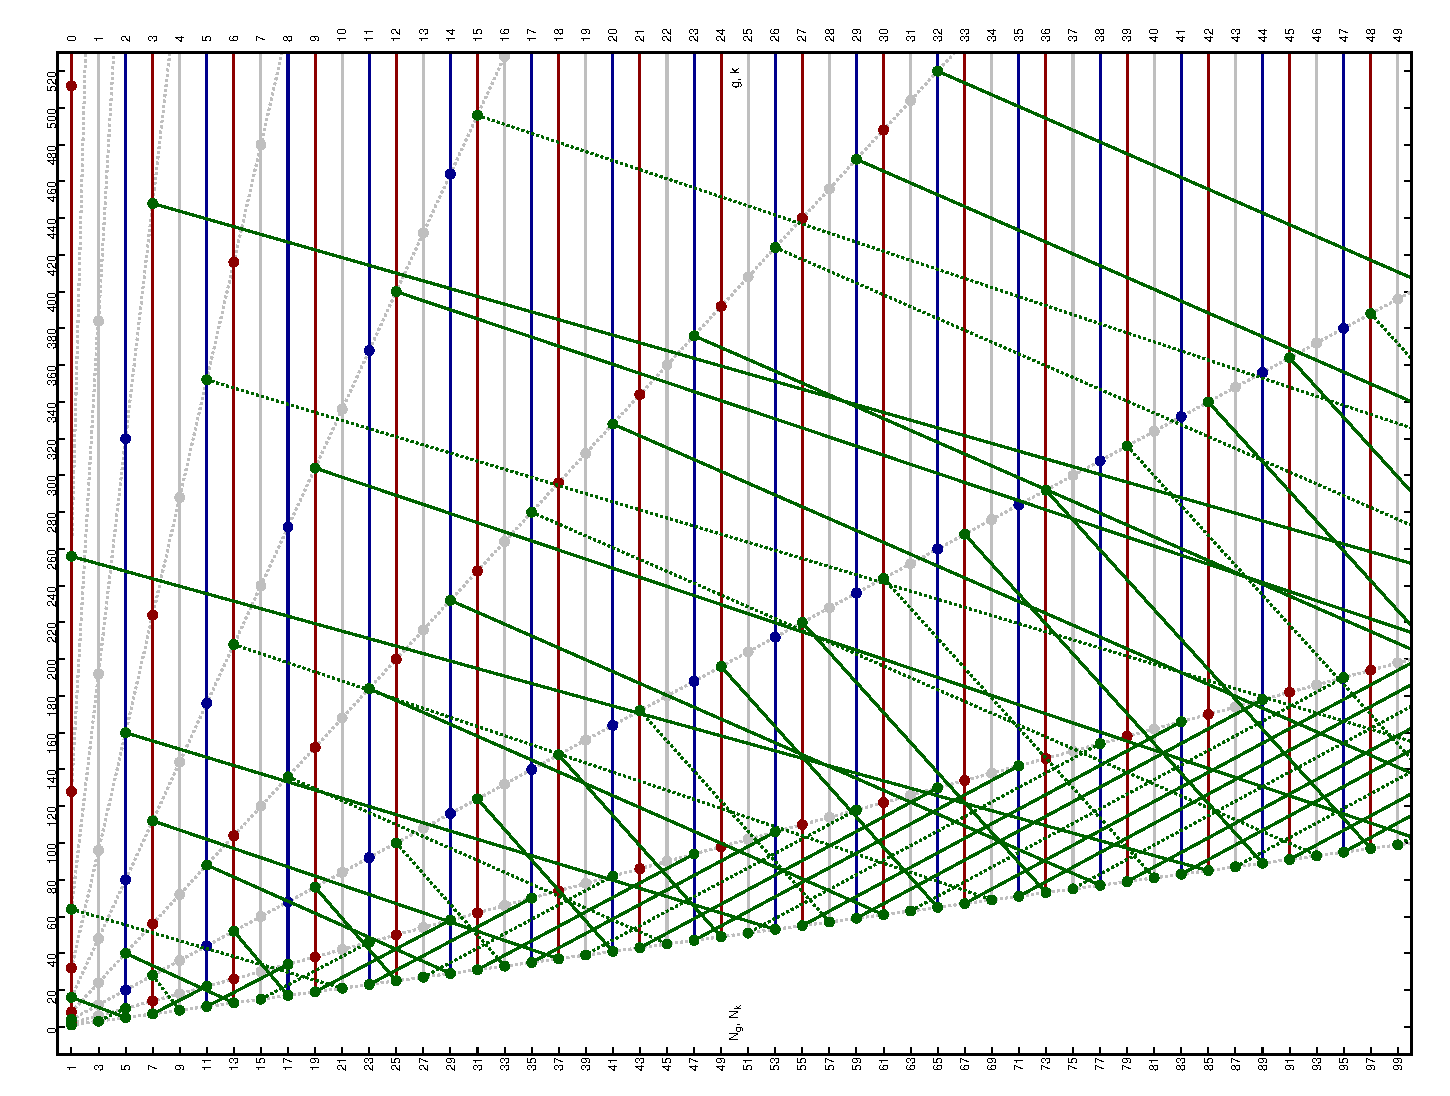
\includegraphics[width= \paperwidth,angle=-90,keepaspectratio]{collatz_flow.eps}
	\caption{$N_g$-$A_k$-$N_k$ relation, best viewed in landscape orientation}
\label{fig:flow}
\end{figure}

Note that, while in the reverse path the position of $A_k$ in the diagram is unambiguous, in the forward path Eq. \ref{eq:geneq} cannot be solved easily without using complex numbers.

%-----------------------------------------------------------------------------
\subsection{Interpretation in terms of $n$}
%-----------------------------------------------------------------------------
Eq. \ref{eq:Ak_vs_all} can be interpreted as a scan for all $A_k$ resp. $N_k$ (Eq. \ref{eq:geneqkg}) over all odd numbers $2g+1$ starting from $n=1$ row by row and there must exist an $(g,n)$-pair for every $k$.

By resolving Eq. \ref{eq:Ak_vs_all} for $n=1,2,3$ we define 3 sets $S^{(n)}$. They represent the odd-to-odd connection in the reverse path for a given $n$. table \ref{table:nsetsplit} shows the resolved equation and parametric equations with independent variable $u=0,1,2,3,\ldots$. $S^{(h)}$ was generated by numerical analysis of the linear equations of $S^{(n)}$. As all downward connections $g>k$ are already occupied by $S^{(1)}$, $S^{(h)}$ can only have upward connections $g<k$. According to Wolfram Alpha, $g(u)$ toggles between $3u$ and $3u+2$ with increasing $n$.

\begin{table}[!htbp]
\centering
\begin{tabular}{|l|l|l|l|l|l|l|l|l|}
\hline
	Set & $n$ & Eq. \ref{eq:Ak_vs_all} & $g(u)$ & $k(u)$ & $g$ to $k$ & $N_g(u)$ & $N_k(u)$ & occupied $k$ \\
\hline
	$S^{(1)}$ & $1$      & $3k=2g-1$ & $3u+2$ & $2u+1$ & $g>k$ & $6u+5$ & $4u+3$   & $1,3,5,7,9,\ldots$ \\
	$S^{(2)}$ & $2$      & $3k=4g$   & $3u$   & $4u$   & $g<k$ & $6u+1$ & $8u+1$   & $4,8,12,16,\ldots$ \\
	$S^{(3)}$ & $3$      & $3k=8g+2$ & $3u+2$ & $8u+6$ & $g<k$ & $6u+5$ & $16u+13$ & $6,14,22,30,\ldots$ \\
	$S^{(h)}$ & $\ge4$   &           &        & $8u+2$ & $g<k$ &        & $16u+5$  & $2,10,18,26,\ldots$ \\
\hline
\end{tabular}
	\caption{Splitting the reverse path connections into 3+1 sets $S^{(n)}$ for $n=1,2,3$ and $S^{(h)}$ for $h=n\ge4$}.
\label{table:nsetsplit}
\end{table}

We can further split the sets of reverse path connections $S^{(n)}$ and $S^{(h)}$ into 12 sets $S^{(nC)}$ and $S^{(hC)}$, with $n$ as before and $C$ being the destination color (Table \ref{eq:color_cases}) of the connection. The per-color index is $s=0,1,2,3\ldots$.
\begin{table}[!htbp]
\centering
\begin{tabular}{|l|l|l|l|l|}
\hline
	Set & $n$ & C-Map & Src & Dst  \\
\hline
	$S^{(1G)}$ & $1$ & $\textcolor{blue}{B_s} \mapsto G_s$ & $3s$   & $2s$   \\
	$S^{(1R)}$ & $1$ & $\textcolor{blue}{B_s} \mapsto \textcolor{red}{R_s}$ & $3s+1$ & $2s+1$ \\
	$S^{(1B)}$ & $1$ & $\textcolor{blue}{B_s} \mapsto \textcolor{blue}{B_s}$ & $3s+2$ & $2s+1$ \\
	$S^{(2R)}$ & $2$ & $\textcolor{red}{R_s} \mapsto \textcolor{red}{R_s}$ & $3s$   & $4s$   \\
	$S^{(2G)}$ & $2$ & $\textcolor{red}{R_s} \mapsto G_s$ & $3s+1$ & $4s+1$ \\
	$S^{(2B)}$ & $2$ & $\textcolor{red}{R_s} \mapsto \textcolor{blue}{B_s}$ & $3s+2$ & $4s+2$ \\
	$S^{(3R)}$ & $3$ & $\textcolor{blue}{B_s} \mapsto \textcolor{red}{R_s}$ & $3s$   & $8s+2$ \\
	$S^{(3B)}$ & $3$ & $\textcolor{blue}{B_s} \mapsto \textcolor{blue}{B_s}$ & $3s+1$ & $8s+4$ \\
	$S^{(3G)}$ & $3$ & $\textcolor{blue}{B_s} \mapsto G_s$ & $3s+2$ & $8s+7$ \\
	$S^{(hR)}$ & $\ge4$ & $?\mapsto \textcolor{red}{R_s}$ & $?$   & $8s+6$ \\
	$S^{(hG)}$ & $\ge4$ & $?\mapsto G_s$ & $?$ & $8s+3$ \\
	$S^{(hB)}$ & $\ge4$ & $?\mapsto \textcolor{blue}{B_s}$ & $?$ & $8s$ \\
\hline
\end{tabular}
	\caption{Subsets of reverse path connections per destination color}
\label{table:nsetcolorsplit}
\end{table}

%-----------------------------------------------------------------------------
\section{Relation between odd numbers}
%-----------------------------------------------------------------------------
Diagram \ref{fig:S_tree} shows the mapping between $g$ and $k$ using table \ref{table:nsetsplit}. The $x$-axis corresponds to the $N_k$-axis of Fig. \ref{fig:flow} and vertical connections correspond to the lines of sets R and B. Connections to members of set G can be handled as endpoints and are shown as gray circles. Pink connections are the open entry points for $n\ge4$.

\begin{figure}[!htbp]
  \centering
	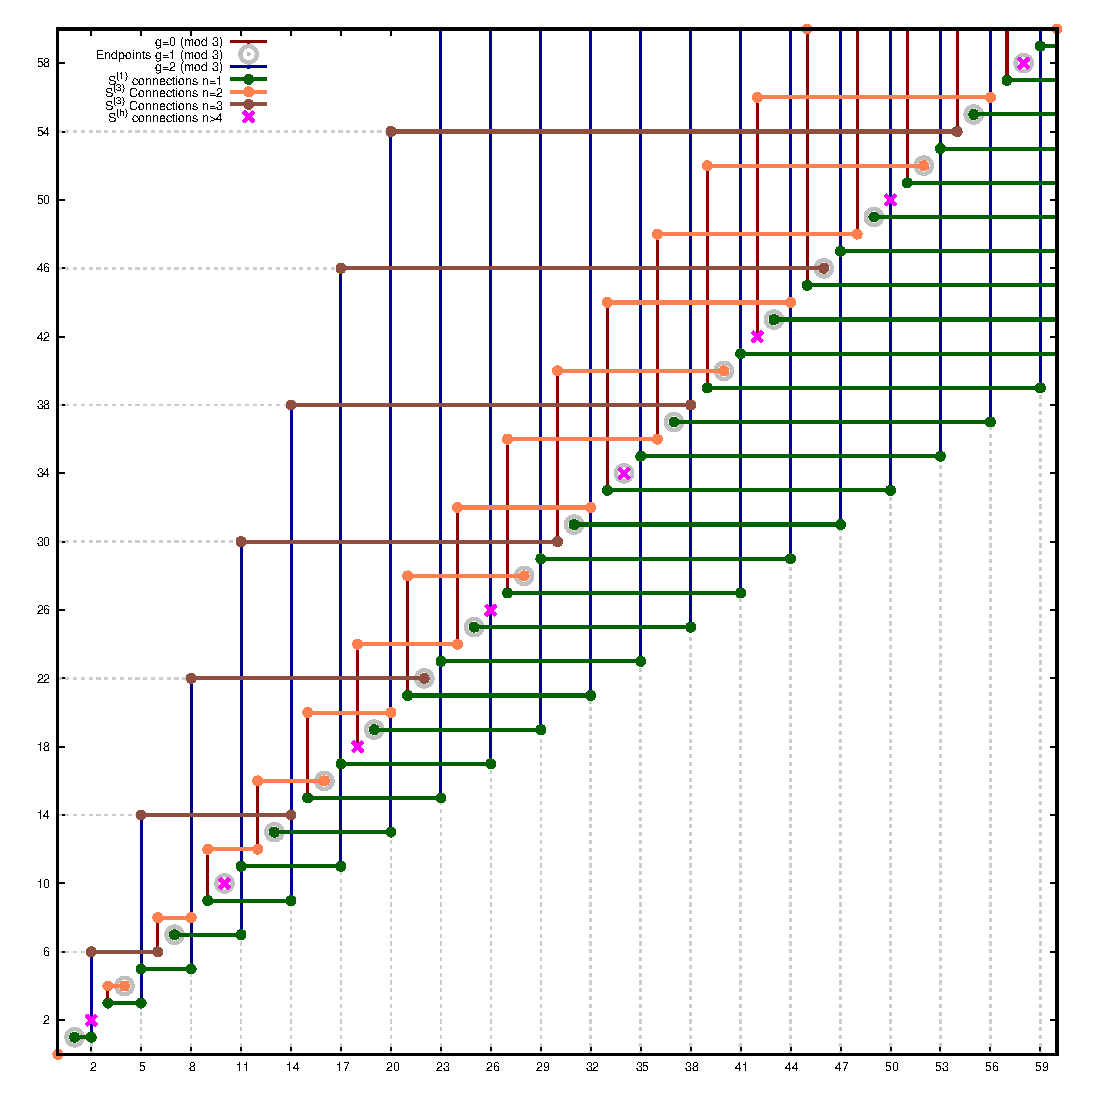
\includegraphics[width= \textwidth,keepaspectratio]{collatz_S_tree.eps}
	\caption{g-k connections}
\label{fig:S_tree}
\end{figure}

The graph shows that all open connections are endpoints and/or connect to the set $S^{(h)}$. As any connection in $S^{(h)}$ connects strictly from left ($g<k$), we can iterate over all $S^{(h)}$ points and close the open connections.

%-----------------------------------------------------------------------------
\subsection{Proposed solution using graph theory}
%-----------------------------------------------------------------------------
By further splitting and/or using the same base (2 or 3) for $g$ and $k$ in table \ref{table:nsetsplit} resp. Src and Dst in table \ref{table:nsetcolorsplit} the mapping could be translated to some kind of adjacency matrix and/or be solved by iteration.
The distinction between $S^{(n)}$ and $S^{(h)}$ seems to be reasonable in the way that within $n<4$ the connections per $N_g$ are limited to 2 in set R and 3 in set B. Also there is no mapping from $1$ within that range (except the self-mapping at $1$).

The paths to the endpoints could be shortened succesively to get a simpler graph.

%-----------------------------------------------------------------------------
\subsection{Other possible solutions}
%-----------------------------------------------------------------------------
\begin{asparaitem}
\item The equations in \ref{table:nsetsplit} can be grouped to vectors on which rotation and shift operations are applied so there might be a solution using linear algebra.
\item Fig. \ref{fig:flow} shows that $A_k$ splits the set of odd numbers into periodic intervals. 
\item Some mapping to complex numbers could handle the rotation.
\end{asparaitem}

We suggest to handle $n=1,2,3$ separately using graph theory, although in terms of intervals there is no such distinction.
%-----------------------------------------------------------------------------
\section{Summary}
%-----------------------------------------------------------------------------
It has been shown that the reverse tree started from $1$ has only the trivial cycle. If there already exists a proof that all odd numbers are connected somehow, the provided lemmas show that the reverse tree is built without gaps or loops.

%-----------------------------------------------------------------------------
\section{Acknowledgements}
%-----------------------------------------------------------------------------
Thank you!

%-----------------------------------------------------------------------------
\section{Sources}
%-----------------------------------------------------------------------------
Additional material used for generating the graphs with gnuplot can be found on

\url{https://github.com/maaaax/collatz}

\end{document}
